\documentclass[12pt]{article}

\usepackage[utf8]{inputenc}
\usepackage[T1]{fontenc}  
\usepackage{hyperref}    
\usepackage{url}   
\usepackage{graphicx}
\usepackage{tabularx}
\usepackage{mathptmx}
\usepackage[romanian]{babel}
\usepackage{indentfirst}
\usepackage{subfig}

\graphicspath{ {./graphics/} }

\hypersetup{
	colorlinks=true,
	linkcolor=blue,
	filecolor=magenta,      
	urlcolor=cyan,
}
\urlstyle{same}

\newcolumntype{C}[1]{>{\centering\arraybackslash}p{#1}}


\title{\textbf{Raport intermediar - Automatic 2D-to-3D image conversion}}

\author{
 	ECHIPĂ: E6
	\\
	 Beldiman Vladislav Student1
	\\
	Grupa 1305A
}

\begin{document}

\noindent\begin{minipage}{0.1\textwidth}
	
\includegraphics[width=1.1cm]{logo_AC.png}
\end{minipage}
\hfill
\begin{minipage}{1\textwidth}\raggedright
	Universitatea Tehnică "Gheorghe Asachi" din Iași\\
	Facultatea de Automatică și Calculatoare\\
	Prelucrarea Imaginilor - Proiect
\end{minipage}

\vspace{5cm}
{\let\newpage\relax\maketitle}
\newpage

\section{Descrierea temei}

Obiectivul acestui proiect este de a crea o aplicație Windows cu interfață grafică care realizează conversia unei imagini din 2D în 3D cu interacțiune minimă în cadrul acestui proces din partea utilizatorului. Acest lucru va fi realizat considerând intensitatea fiecărui pixel drept valoarea înălțimii acestuia într-un câmp de înălțimi, iar pe baza acestor valori va fi construită o plasă poligonală cu fețe triunghiulare (Figura \ref{fig:fig1}).

Aplicația va fi scrisă în limbajul de programare C++ cu interfața grafică realizată cu ajutorul setului de instrumente Qt, iar plasa poligonală va fi sintetizată folosind interfața pentru programarea aplicațiilor OpenGL. Ea va permite vizualizarea imaginii încărcate și finale, cât și salvarea imaginii 3D în format STL.

Utilizatorul va avea la dispoziție următoarele opțiuni pentru calibrarea rezultatului final:
\begin{itemize}
	\item Selectarea algoritmului de triangulație;
	\item Selectarea erorii maxime la triangulație (unde e cazul);
	\item Inversarea imaginii finale (răsturnarea valorilor din câmp);
	\item Adăugarea unui chenar cu grosime și înălțime configurabile la imaginea finală;
	\item Adăugarea unei baze la imaginea finală cu înălțime configurabilă;
	\item Selectarea înălțimii dintre valoarea maximă și minimă de gri.
\end{itemize}

Triangulația domeniului determinat de pixeli va fi realizată prin triangulația naivă (Figura \ref{fig:fig2}) care include toate punctele corespunzătoare pixelilor, sau prin aproximare prin înserare lacomă (Figura \ref{fig:fig3}) aplicând triangulația Delaunay sau triangulația dependentă de date cu unele optimizări [1]. Înserarea lacomă va folosi drept măsură de importanță pentru fiecare punct eroarea verticală dintre valoarea câmpului și aproximarea interpolată în acel punct.

\begin{figure}[!htb]
	\begin{minipage}{0.32\textwidth}
		\centering
		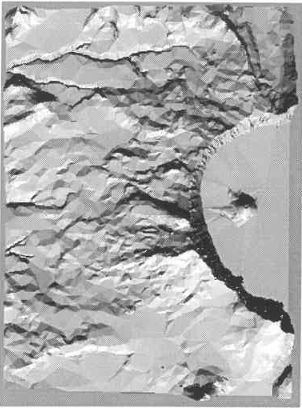
\includegraphics[width=.7\linewidth]{ExempluPlasa.png}
		\caption{Exemplu de plasă poligonală rezultantă. [1]}\label{fig:fig1}
	\end{minipage}\hfill
	\begin{minipage}{0.32\textwidth}
		\centering
		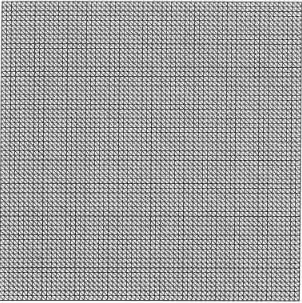
\includegraphics[width=.7\linewidth]{ExempluTriangulatieNaiva.png}
		\caption{Exemplu de triangulație naivă. [1]}\label{fig:fig2}
	\end{minipage}\hfill
	\begin{minipage}{0.32\textwidth}
		\centering
		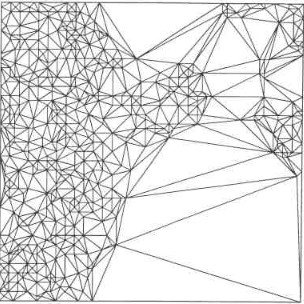
\includegraphics[width=.7\linewidth]{ExempluTriangulatieCuAproximari.png}
		\caption{Exemplu de triangulație care aproximează un câmp de înălțimi. [1]}\label{fig:fig3}
	\end{minipage}
\end{figure}

\newpage
\vspace{10cm}
\section{Modalitatea de lucru propusă}%\textsuperscript{\tiny1}}

\textbf{Git repository:} \url{https://github.com/veeyslaw/hfbm}

\begin{center}
	\begin{tabular}{|C{0.3cm}|C{10cm}|C{2cm}|C{2cm}|} 
		\hline
		\textbf{\#} & \textbf{Descriere sarcină} & \textbf{Stare} & \textbf{Membru} \\ 
		\hline
		1 & Documentare despre conversia imaginilor din 2D în 3D & în progres &  m1 \\ 
		\hline
		2 & Documentare despre Qt & în progres &  m1  \\ 
		\hline
		3 & Documentare despre OpenGL & în progres &  m1  \\ 
		\hline
		4 & Implementarea și testarea unei interfețe grafice minimaliste & încheiată &  m1 \\ 
		\hline
		5 & Implementarea și testarea algoritmului naiv & încheiată &  m1 \\ 
		\hline
		6 & Documentare despre formatul StL & încheiată &  m1 \\
		\hline
		7 & Implementarea și testarea opțiunii de salvare în format StL a imaginii 3D & încheiată &  m1 \\
		\hline
		8 & Întocmirea raportului intermediar & încheiată &  m1 \\
		\hline
		9 & Extinderea interfeței grafice cu opțiuni de calibrare și perfectarea acesteia & în progres &  m1 \\
		\hline
		10 & Implementarea și testarea opțiunilor de calibrare & - &  m1 \\
		\hline
		11 & Implementarea și testarea algoritmului bazat pe triangulația Delaunay & - &  m1 \\
		\hline
		12 & Implementarea și testarea algoritmului bazat pe triangulația dependentă de date & - &  m1 \\
		\hline
		13 & Rafinare și optimizări & în progres &  m1 \\ 
		\hline
		14 & Identificarea unui set potrivit de imagini (preferabil găsirea unei surse cu rezultate experimentale împreună cu probele folosite) & - & m1 \\
		\hline
		15 & Adăugarea posibilității de cronometrare a timpului de conversie & - &  m1 \\ 
		\hline
		16 & Realizarea experimentelor & - &  m1 \\ 
		\hline
		17 & Întocmirea raportului final & - &  m1 \\ 
		\hline
		18 & Pregătirea prezentării & - &  m1 \\ 
		\hline
	\end{tabular}
\end{center}

%{\tiny\textsuperscript{1}Unele sarcini, precum documentarea, nu vor fi realizate decât la finalul proiectului.}

\section{Rezultate și concluzii}

\subsection{Implementarea și testarea unei interfețe grafice minimaliste}

Interfața grafică a fost implementată cu ajutorul setului de intrumente Qt. În timpul implementării am realizat faptul că QMesh - clasa pentru un încărcător de plase personalizate pe care intenționam să o folosesc - nu oferă la fel de multe facilități la câte mă așteptam. Astfel, am decis să folosesc OpenGL pentru sintetizarea plasei prin interfața oferită de Qt într-un QOpenGLWidget.

La acest pas interfața permitea încărcarea și vizualizarea imaginii de intrare încărcate într-un QLabel și vizualizarea plasei rezultante care permite și scalarea ei cu ajutorul roții șoricelului, cât și rotirea aceasteia pe axa Ox și Oy. De asemenea, au fost conectate butoanele adăugate la funcțiile corespunzătoare care urmau să fie implementate.

Rezultate: Figura \ref{fig:fig4}

\begin{figure}[!htb]
	\begin{minipage}{0.48\textwidth}
		\centering
		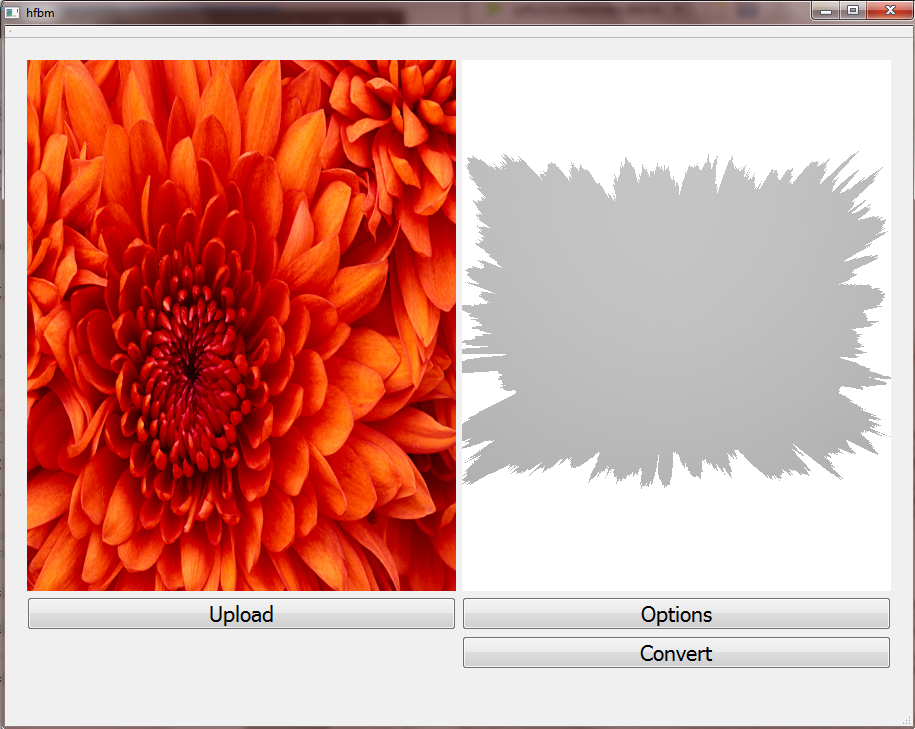
\includegraphics[width=.7\linewidth]{PrimaPaginaInterfata1.png}
		\caption{Pagina principanlă după prima etapă.}\label{fig:fig4}
	\end{minipage}\hfill
	\begin{minipage}{0.32\textwidth}
		\centering
		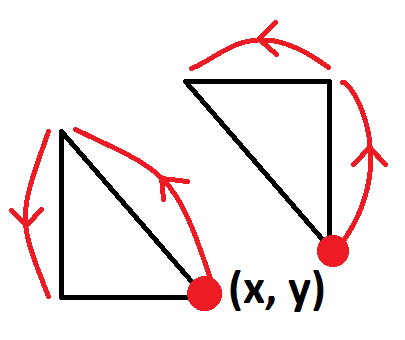
\includegraphics[width=.7\linewidth]{NaivaOrdine.png}
		\caption{Alegerea triunghiurilor triangulația naivă.}\label{fig:fig5}
	\end{minipage}\hfill
\end{figure}

\subsection{Implementarea și testarea algoritmului naiv}

Algoritmul naiv a fost implementat și testat cu succes. În cadrul algoritmului este adăugat câte un punct pentru fiecare punct din imaginea sursă având ca valoare pe axa Oz valoarea de gri a imaginii normalizată. După care, pentru fiecare punct în afară de cele de pe prima coloană și primul rând sunt adăugate câte 2 triunghiuri în tabloul de indici după cum e prezentat în figura \ref{fig:fig5}.

Rezultate: Figurile \ref{fig:fig6} \ref{fig:fig7}

\begin{figure}[!htb]
	\begin{minipage}{0.48\textwidth}
		\centering
		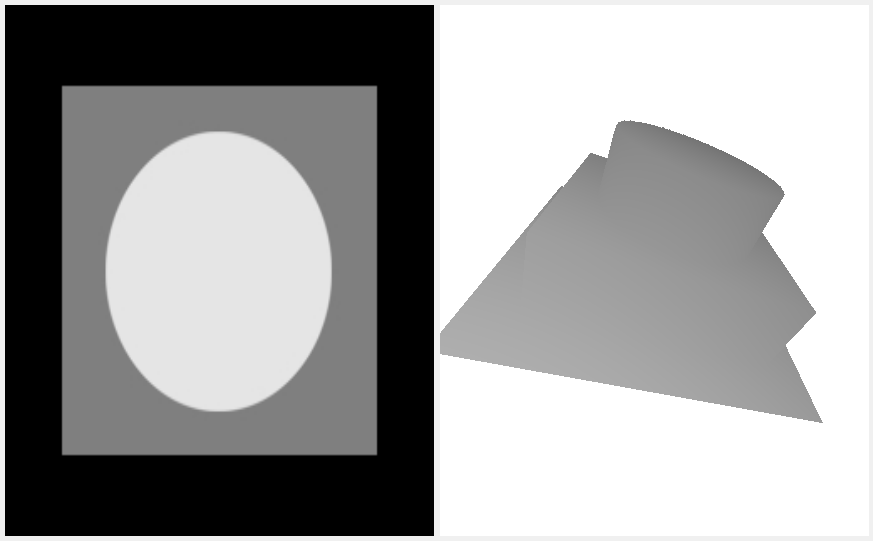
\includegraphics[width=.7\linewidth]{ExempluNaiva1.png}
		\caption{Exemplu triangulație naivă 1.}\label{fig:fig6}
	\end{minipage}
	\begin{minipage}{0.48\textwidth}
		\centering
		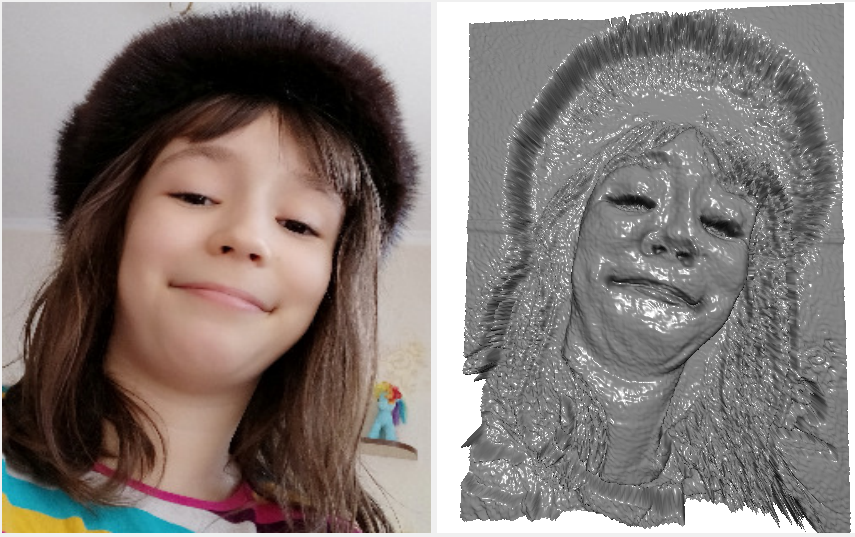
\includegraphics[width=.7\linewidth]{ExempluNaiva2.png}
		\caption{Exemplu triangulație naivă 2.}\label{fig:fig7}
	\end{minipage}\hfill
\end{figure}

\subsection{Implementarea și testarea opțiunii de salvare în format StL a imaginii 3D}

În timpul rezolvării acestei sarcini, cât și a documentării despre OpenGL, am stabilit cum vor fi stocate datele plasei în timpul triangulației și după, și anume: coordonatele punctelor într-un vector de tridimensional, la care va fi adăugată după finisarea algoritmului date despre culorile și normalele cu scopul de a le sintetiza în QOpenGLWidget, iar în loc de a stoca majoritatea punctelor de 2 ori, va fi folosit un tablou de indici, câte 3 pentru fiecare triunghi, fiecare din ei reprezentând poziția în tabloul de puncte a punctelor care îl alcătuiesc, eliminând nevoia de a stoca câte 2 puncte pentru fiecare latură comună din plasă. În plus, OpenGL ne permite să folosim și această reprezentare la tamponarea datelor pentru sintetizare. Indicii vor apărea în ordine trigonometrică, ordine conformă cu standardul StL [2], și cu modul implicit în care detectează OpenGL orientarea triunghiurilor.

Conform standardului StL [2]:
\begin{itemize}
	\item Un fișier StL constă dintr-o listă de date despre fațete;
	\item Orientarea fațetelor e specificată redundant în două moduri - prin direcția normalei și prin ordinea în care sunt specificate vârfurile - trigonometrică;
	\item Fiecare triunghi trebuie să împartă două vârfuri cu fiecare două triunghiuri vecine;
	\item Formatul binar e compus dintr-un antet pe 80 de bytes care nu are nici o semnificație de dată, 4 bytes de tipul unsigned long integer - numărul de fațete în fișier, după care pentru fiecare triunghi sunt adăugate datele: 3 x 4 bytes de tip float care reprezintă vectorul normalei, câte 3 x 4 bytes de tip float pentru toți cei 3 vectori - vârfuri, și 2 bytes de tip unsigned integer care nu vor avea vreo însemnătate în cadrul proiectului;
\end{itemize}

Rezultate: Figura \ref{fig:fig8} (Rezultatul e prezentat într-un \href{https://www.viewstl.com/}{vizualizator StL online}, deoarece încărcarea unui fișier StL și vizualizarea acestuia nu se include în scopul proiectului.)

\begin{figure}[!htb]
	\begin{minipage}{0.48\textwidth}
		\centering
		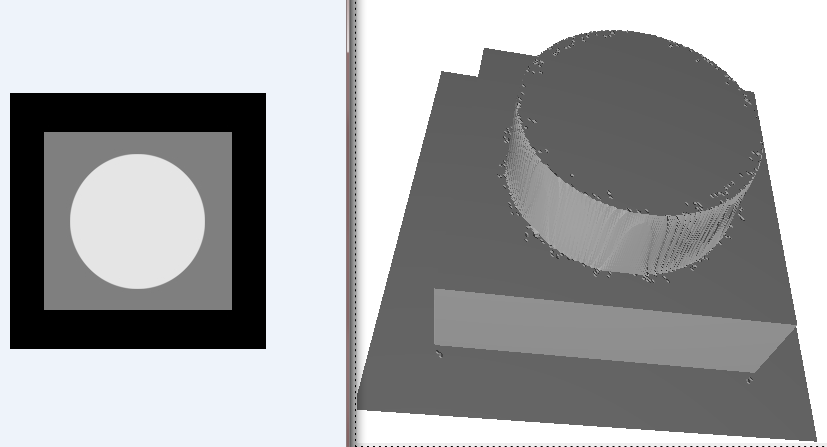
\includegraphics[width=.7\linewidth]{ExempluSalvare.png}
		\caption{Exemplu salvare și afișare în altă \href{https://www.viewstl.com/}{aplicație.}}\label{fig:fig8}
	\end{minipage}
	\begin{minipage}{0.48\textwidth}
		\centering
		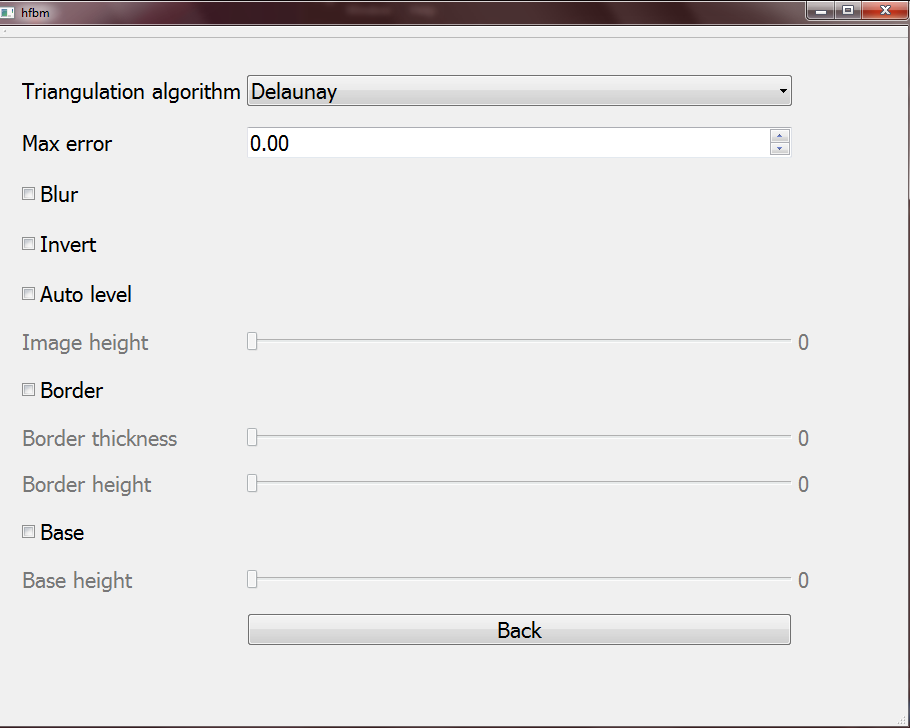
\includegraphics[width=.7\linewidth]{DouaPaginaInterfata.png}
		\caption{Pagina cu opțiuni curentă.}\label{fig:fig9}
	\end{minipage}\hfill
\end{figure}

\subsection{Extinderea interfeței grafice cu opțiuni de calibrare și perfectarea acesteia}

A fost adăugată cea mai mare parte a interfeței grafice pentru selectarea opțiunilor de calibrare (Figura \ref{fig:fig9}). 

\subsection{Implementarea și testarea opțiunilor de calibrare}

-

% Rezultate: Figura \ref{fig:fig4}

\subsection{Implementarea și testarea algoritmului bazat pe triangulația Delaunay}

-

% Rezultate: Figura \ref{fig:fig4}

\subsection{Implementarea și testarea algoritmului bazat pe triangulația dependentă de date}

-

% Rezultate: Figura \ref{fig:fig4}

\subsection{Identificarea unui set potrivit de imagini (preferabil găsirea unei surse cu rezultate experimentale împreună cu probele folosite)}

-

% Rezultate: Figura \ref{fig:fig4}


\section*{Referințe}

\medskip

[1] \href{http://reports-archive.adm.cs.cmu.edu/anon/anon/home/ftp/1995/CMU-CS-95-181.pdf} {Garland M. and Heckbert P. S. (1995) Fast Polygonal Approximation of Terrains and Height Fields. (CMU-CS-95-181)}

[2] \href{https://www.fabbers.com/tech/STL_Format#Sct_binary} {Marshall Burns. Automated Fabrication
Improving Productivity in Manufacturing.}

\end{document}